\section{Decision Procedures} \label{decision_procedures}

Given a theory $\mathcal{T}$ in a formula $\psi$ in 
the language of the theory, is it possible to know 
$\models_{\mathcal{T}} \psi$? The last question is 
known as the verification of the decision problem for 
the respective theory $\mathcal{T}$. This question has 
been studied extensively for many theories of interest 
\cite{borger2001classical}. 

Regarding the decidability of the theories 
mentioned in Section \ref{math_theories}, it is known that 
EUF is undecidable \cite{borger2001classical}, and the theory
of ordered commutative rings is undecidable when the
structure uses integers as the domain and the semantics
of the arithmetical operations \cite{DBLP:books/daglib/0076838} 
(on the other hand, this theory can be decidable if we
keep the same structure but use the reals as the domain
\cite{DBLP:books/daglib/0076838}).
Nonetheless, the quantifier-free fragment of EUF and 
the restriction imposed in the decision problem for 
the UTVPI theory allow efficient algorithms to decide 
validity and satisfiability in their respective theories 
\cite{10.1145/322186.322198, 10.1145/322217.322228, 
10.1007/11559306_9}.

In the rest of this section we review some decision 
problems and provide references to their respective
decision procedures used in the implementation work of 
the thesis.

\subsection{Satisfiability and Satisfiability Modulo Theories}

The satisfiability problem consists of finding a 
propositional assignment for a propositional formula. 
This problem is at the core level of complexity theory, 
defining an important class of problems known as 
NP, which includes problems whose
algorithms seem to be intractable.
Developments in algorithms and heuristics 
\cite{10.5555/2898950, 
935565} have made it possible to use satisfiability 
algorithms 
to solve real-world problems in 
verification \footnote{These
  advances do not provide an answer to the well-known P vs. NP
  problem. There are results indicating a class of problem instances
  for many of the SAT algorithms which cannot be solved in less that
  \bigO{2^n} steps \cite{10.5555/2898950}.
}.

The DPLL algorithm \cite{10.1145/368273.368557} 
(and other extensions) is the algorithm
found in many SAT solvers. Fundamentally, it is a search-based algorithm
which implements operators (decide, unit-propagation, backtrack)
to find a satisfiable assignment. If the algorithm is not able to
find a satisfying assignment for a formula, then it is possible to 
extract a \emph{resolution proof} based on the traces of the search
operations.

\begin{example}

  \begin{figure}

    \centering

    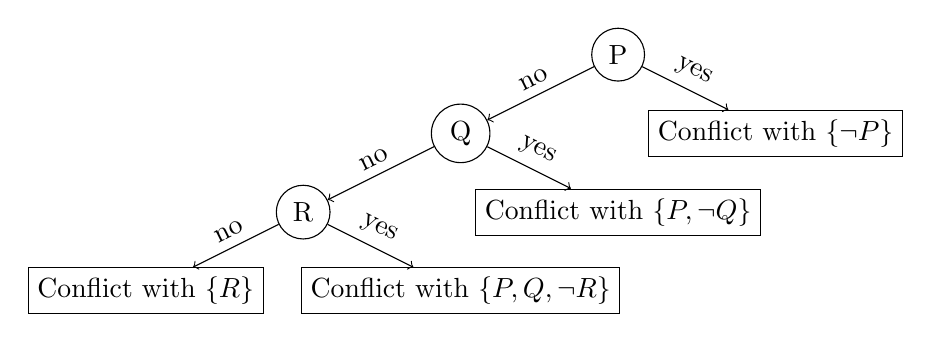
\begin{tikzpicture}[->]
      \node(p) at (6, 5) [circle, draw] {P};
      \node(q) at (4,4) [circle, draw] {Q};
      \node(r) at (2, 3) [circle, draw] {R};
      \node(expl1) at (8, 4) [rectangle, draw] {Conflict with $\{\neg P\}$};
      \node(expl2) at (6, 3) [rectangle, draw] {Conflict with $\{P, \neg Q\}$};
      \node(expl3) at (4, 2) [rectangle, draw] {Conflict with $\{P, Q, \neg R\}$};
      \node(expl4) at (0, 2) [rectangle, draw] {Conflict with $\{R\}$};

      \path[every node/.style={sloped,anchor=south,auto=false}]
      (p) edge node {yes} (expl1)   
      (p) edge node {no}  (q)   
      (q) edge node {yes} (expl2)
      (q) edge node {no}  (r)
      (r) edge node {yes} (expl3)
      (r) edge node {no}  (expl4);
    \end{tikzpicture}

    \caption{Example of DPLL execution on 
      $\{\{\neg P\}, \{P, Q, \neg R\}, \{R\}, 
    \{P, \neg Q\} \}$} \label{dpll_figure}

  \end{figure}

  We can see that the following resolution proof resembles the
  structure of the DPLL execution on figure \ref{dpll_figure}, i.e.
  if we rotate the proof-tree and mark the nodes by the pivots used
  we obtained a similar tree obtained by the execution of the DPLL
  algorithm. This fact becomes relevant because it enables us 
  to construct a resolution proof from the traces of a SAT 
  solver used
  in the theory combination part of the implementation. 

  \begin{figure}
    \centering
    \begin{prooftree}
      \hypo[]{\neg P}
      \hypo[]{P \lor Q \lor \neg R}
      \infer2[$res_P$]{Q \lor \neg R}
      \hypo[]{R}
      \infer2[$res_R$]{Q}
      \hypo[]{P \lor \neg Q}
      \infer2[$res_Q$]{P}
      \hypo[]{\neg P}
      \infer2[$res_P$]{\bot}
    \end{prooftree}
    \caption{Example of resolution proof} 
    \label{example_resolution_proof}
  \end{figure}

\end{example}

We can extend this approach to work not only with propositional
variables but with terms of more complex signatures 
\cite{10.5555/1391237}. If we are given a boolean combination 
of formulas from any theory that is capable of deciding the 
satisfiability of any conjunction of formulas in the theory, 
by using a \emph{lazy framework} integration with a SAT solver it is 
possible to find either a model or declare unsatisfiable such boolean
combination as follows: (i) first abstract the literals in the boolean
combination to (pseudo) boolean propositions; (ii) find a satisfying
assignment (using a SAT solver) of the (pseudo) boolean propositions;
(iii) using the theory solver, test if the collection of positive
and negative literals induced by the pseudo boolean variables is
satisfiable; (iv) if it is then declare the formula satisfiable, 
otherwise \emph{learn} (or block) the pseudo boolean clause obtained
(by negating the conjunction of boolean constraints) in the SAT
solver and repeat from step (ii); (v) if it is not possible to
find a satisfying assignment for the pseudo boolean variables, 
declare the original formula to be unsatisfiable.

These algorithms are used in the last section of the thesis work.
The implementation for the interpolation combination method
in \cite{10.1007/11532231_26} requires a resolution-based
proof in order to compute partial interpolants by integrating
Pudlak's algorithm.

%%% Local Variables:
%%% mode: latex
%%% TeX-master: "main"
%%% End:

\subsection{Congruence Closure}

The congruence closure problem consists of given a conjunction of
equalities and disequalities $\psi$ determine if an equality
$u = v$ follows from the consequence generated by $\models_{EUF} 
\psi$.

In \cite{10.1007/978-3-540-32033-3_33}, the authors 
introduced a Union-Find data structure that supports the 
Explanation operation. This operation receives as input 
an equation between constants. If the input equation is 
a consequence of the current equivalence relation defined 
in the Union Find data structure, the Explanation operation 
returns the minimal sequence of equations used to build 
such equivalence relation, otherwise it returns 
`Not provable'. A proper implementation of this algorithm 
extends the traditional Union-Find data structure with 
a \emph{proof-forest}, which consists of an additional 
representation of the underlying equivalence relation that 
does not compress paths whenever a call to the Find 
operation is made. For efficient reasons, the Find 
operation uses the path compression and weighted union.

The main observation in \cite{10.1007/978-3-540-32033-3_33} 
is that, in order to recover an explanation between 
two terms, by traversing the path between the two nodes 
in the proof tree, the last edge in the path guarantees to 
be part of the explanation. Intuitively, this follows because only 
the last Union operation was responsible of merging the 
two classes into one. Hence, we can recursively recover 
the rest of the explanation by recursively traversing 
the subpaths found.

Additionally, the authors in \cite{10.1007/978-3-540-32033-3_33} 
extended the Congruence Closure algorithm 
\cite{10.1007/978-3-540-39813-4_5} using the above data 
structure to provide Explanations for the theory of EUF. The congruence 
closure algorithm is a simplification of the congruence 
closure algorithm in \cite{10.1145/322217.322228}. The latter 
combines the traditional \emph{pending} and \emph{combine} list 
into one single list, hence removing the initial 
\emph{combination} loop in the algorithm in 
\cite{10.1145/322217.322228}.

%%% Local Variables:
%%% mode: latex
%%% TeX-master: "main"
%%% End:

\subsection{Satisfiability of Horn clauses of propositions and grounded equations}

TODO.

\subsubsection{Decision Problem}

TODO.

\subsubsection{Decision Procedure}

In \cite{GALLIER1987233} it was proposed an algorithm 
for testing the unsatisfiability
of ground Horn clauses with equality. The main idea was 
to interleave two algorithms: \emph{implicational propagation}
(propositional satisfiability of Horn clauses) that 
updates the truth value of equations in the antecedent 
of the input Horn clauses \cite{DOWLING1984267}; and 
\emph{equational propagation} (congruence closure for 
grounded equations) to update the state of a 
Union-Find data structure \cite{10.1145/364099.364331}
that keeps the minimal equivalence relation defined 
by grounded equations in the input Horn clauses.

The author in \cite{GALLIER1987233} defined two 
variations of his algorithms by adapting
the Congruence Closure algorithms in 
\cite{10.1145/322217.322228, 10.1145/322186.322198}.
Additionally, modifications in the data structures 
used by the original algorithms were needed
to make the interleaving mechanism more efficient.

TODO.

%%% Local Variables:
%%% mode: latex
%%% TeX-master: "main"
%%% End:

\subsection{Nelson-Oppen framework for theory and interpolation
combination}

The theory combination problem consists on taking a 
formula from the union of two (or more) disjoint 
languages and tell if such formula is satisfiable
or not in the combined theory, i.e. a theory resulting
after putting together two (or more) axiomatizations.

In \cite{10.1145/357073.357079} the authors defined a procedure
to achieve the above problem. The key idea is to \emph{purify} 
the sub-formulas by including additional constant 
symbols equating sub-terms such that the resulting formula 
can be splitted into components of the appropriate language 
for each theory solvers to work with. The separation naturally
will hide relevant information to the solvers, and they 
might not be able to decide satisfiability correctly.
The authors noticed that to solve the above problem it is enough to 
share disjunction of equalities between the combined theories of shared
terms. In addition, they proved that some theories have the 
following property:

\begin{definition}
  Let $\mathcal{T}$ be a theory. We say that $\mathcal{T}$
  is a \emph{convex theory} if a finite conjunction of formulas 
  in $\mathcal{T}$ $\psi = \bigwedge_{i = 1}^m \psi_i$ satisfies
  $\psi \models_{\mathcal{T}} \bigvee_{j = 1}^n 
  x_j = y_j$, then exists $k \in \{1, \dots, n \}$ such that 
  $\psi \models_{\mathcal{T}} x_k = y_k$.
\end{definition}

Hence, it is important to detect
whether the theories involved are convex or not since 
this can improve performance since convex theories do not
need to share disjunctions of equalities as mentioned before
(since all these disjunctions imply a single equality).

\begin{example}
  \begin{itemize}
    \item The conjunctive fragment of equality logic is an example
      of a convex theory since
      it can always decide the membership of an equation in the 
      equivalence relation. 
    \item The theory of UTVPI over the integers is an example of 
      non-convex theory. To see the latter consider
      $1 \leq x \land x \leq 2 \models_{UTVPI(\mathbb{Z})} 1 = x \lor 2 = x$.
      However, it is not the case that 
      $1 \leq x \land x \leq 2 \models_{UTVPI(\mathbb{Z})} 1 = x$
      nor 
      $1 \leq x \land x \leq 2 \models_{UTVPI(\mathbb{Z})} 2 = x$.
  \end{itemize}
\end{example}

An interpolation combination framework as proposed in \cite{10.1007/11532231_26}
follow the same idea towards theory combination. Inductively, they define
\emph{partial interpolants} for each shared equality/disjunction of equalities
until some theory reaches the unsatisfiable state, which is expected since 
an interpolant is a pair a mutually contradicting formulas.

This framework was implemented in the thesis work. This framework was chosen
in particular since it allows working with non-convex theories (in our case
for the theory of UTVPI over $\mathbb{Z}$).

%%% Local Variables:
%%% mode: latex
%%% TeX-master: "main"
%%% End:


%%% Local Variables:
%%% mode: latex
%%% TeX-master: "main"
%%% End:
